\documentclass{beamer}

\usepackage{graphicx,hyperref,udesc,url}
\usepackage[latin1]{inputenc}
\usepackage{bussproofs}
%\usepackage[T1]{fontenc}
\usepackage{booktabs}
\usepackage[portuges]{babel}

\AtBeginSection[]{
  \begin{frame}[noframenumbering]
  \vfill
  \centering
  \begin{beamercolorbox}[sep=8pt,center,shadow=true,rounded=true]{title}
    \usebeamerfont{title}\insertsectionhead\par%
  \end{beamercolorbox}
  \vfill
  \end{frame}
}

\newcommand\Wider[2][3em]{%
\makebox[\linewidth][c]{%
  \begin{minipage}{\dimexpr\textwidth+#1\relax}
  \raggedright#2
  \end{minipage}%
  }%
}

\title[Extraction of Programs from Proofs]{Programming = Mathematics + Murphy's Law\\ - (E. Dijkstra)}

\author[Rafael Castro, Karina Roggia]{
    Rafael Castro\\\medskip
    {\small \url{rafaelcgs10@gmail.com}}\\\medskip
    Karina Roggia\\\medskip
    {\small \url{karina.roggia@udesc.br}}
  }

\date{04/09/2019}

\begin{document}

\begin{frame}
  \titlepage

\end{frame}

\section{Mini-bibliografia}

\begin{frame}
  \frametitle{Quem foi Edsger Dijkstra?}
  \begin{columns}
    \begin{column}{.555555\textwidth}
      \begin{itemize}
      \item Nome Completo: Edsger Wybe Dijkstra.
      \item Nacionalidade: Holand�s.
      \item Longevidade: 1930 - 2002.
      \end{itemize}
    \end{column}
    \begin{column}{.555555\textwidth}
      \begin{figure}
        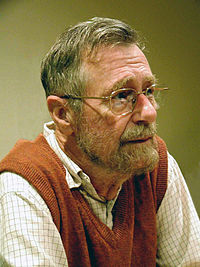
\includegraphics[width = 0.7\textwidth]{dijkstra.jpg}
      \end{figure}
    \end{column}
  \end{columns}
\end{frame}

\begin{frame}
  \frametitle{Alguns trabalhos de Edsger Dijkstra}
  \begin{itemize}
  \item Algoritmo de caminho m�nimo em grafos e redescobriu o algoritmo Prim.
  \item Sistema Operacional THE, tipo BATCH, com camadas de abstra��o e suporte a multitasking.
  \item Vari�vel de sem�foro.
  \item Trabalhou no primeiro compilador da linguagem ALGOL 60.
  \item Introduziu o conceito de pilha em programas recursivos.
  \item Pai da programa��o estruturada - Uso de subrotinas, la�os de repeti��o etc.
  \item Defensor do uso de metodologias matem�ticas na programa��o - Verifica��o formal.
  \item Identificou e apresentou a solu��o de um problema de exclus�o m\'utua em um sistema concorrente.
  \item Resumindo... fez de tudo.
  \end{itemize}
\end{frame}

\begin{frame}
  \frametitle{Pr�mios que Dijkstra ganhou}
  \begin{enumerate}
  \item Fellow da British Computer Society em 1971.
  \item Membro da Royal Netherlands Academy of Arts and Sciences em 1971.
  \item ACM Turing Award em 1972.
  \item American Academy of Arts and Sciences em 1975.
  \item Fellow da Association for Computing Machinery 1994.
  \end{enumerate}
\end{frame}

\section{Frases de Dijkstra}

\begin{frame}
  \frametitle{Divis�o}
  \begin{itemize}
  \item Frases que todos citam, mas que ningu�m sabe o contexto
  \item Frases falando mal de Engenharia de Software
  \item Frases falando mal de Ensino de C. da Computa��o
  \item Frases falando mal de linguagens de programa��o
  \end{itemize}
\end{frame}

\begin{frame}
  \frametitle{Ci�ncia da Computa��o ...}
  \centering
  \includegraphics[width = 0.7\textwidth]{computer-science-is-.jpg}
  \pause
  \\
  \Large{N�o � do Dijkstra!}
\end{frame}


\end{document}
%%% Local Variables:
%%% mode: latex
%%% TeX-master: t
%%% End:
